\documentclass[a4paper]{article}

% subfile handling packages
\usepackage{subfiles}
\newcommand{\onlyinsubfile}[1]{#1}
\newcommand{\notinsubfile}[1]{}

% document packages
\usepackage[top=1in, bottom=1.25in, left=1.25in, right=1.25in]{geometry}
\usepackage{amsmath}
\usepackage{multicol}
\usepackage{graphicx}
\RequirePackage{ltxcmds}[2010/12/07]
\graphicspath{{./images/}}
\usepackage{float}
\usepackage{amsfonts}

% Document metadata
\title{BPSK system}
\author{ }

\begin{document}
\renewcommand{\onlyinsubfile}[1]{}
\renewcommand{\notinsubfile}[1]{#1}

\maketitle

This document describes the simulation BPSK system in back-to-back configuration. 

\section{Functional Description}

A simplified diagram of the system being simulated is presented in the Figure~\ref{fig:physicalsystem}. The system simulated takes a random binary string and encodes it in an optical bandpass signal, signal that afterwards is decoded in order to re-obtain the original binary string.
\par
The decoding of the optical signal is accomplished by an homodyne receiver, which combines the signal with a local oscillator with a user-determined phase. The homodyne receiver block output is then fed into a block that compares it with the original binary string and computes the Bit Error Rate (BER) along with it's upper and lower bounds for a certain user defined confidence level.

%In broad terms, our QKD simulation is required to be able to send a random bit sequence (the key) by means of an optical signal, accomplish a full key reconstruction from the optical signal and subsequently perform a key security check through the evaluation of the Bit Error Rate (BER).

\begin{figure}[h]
\centering
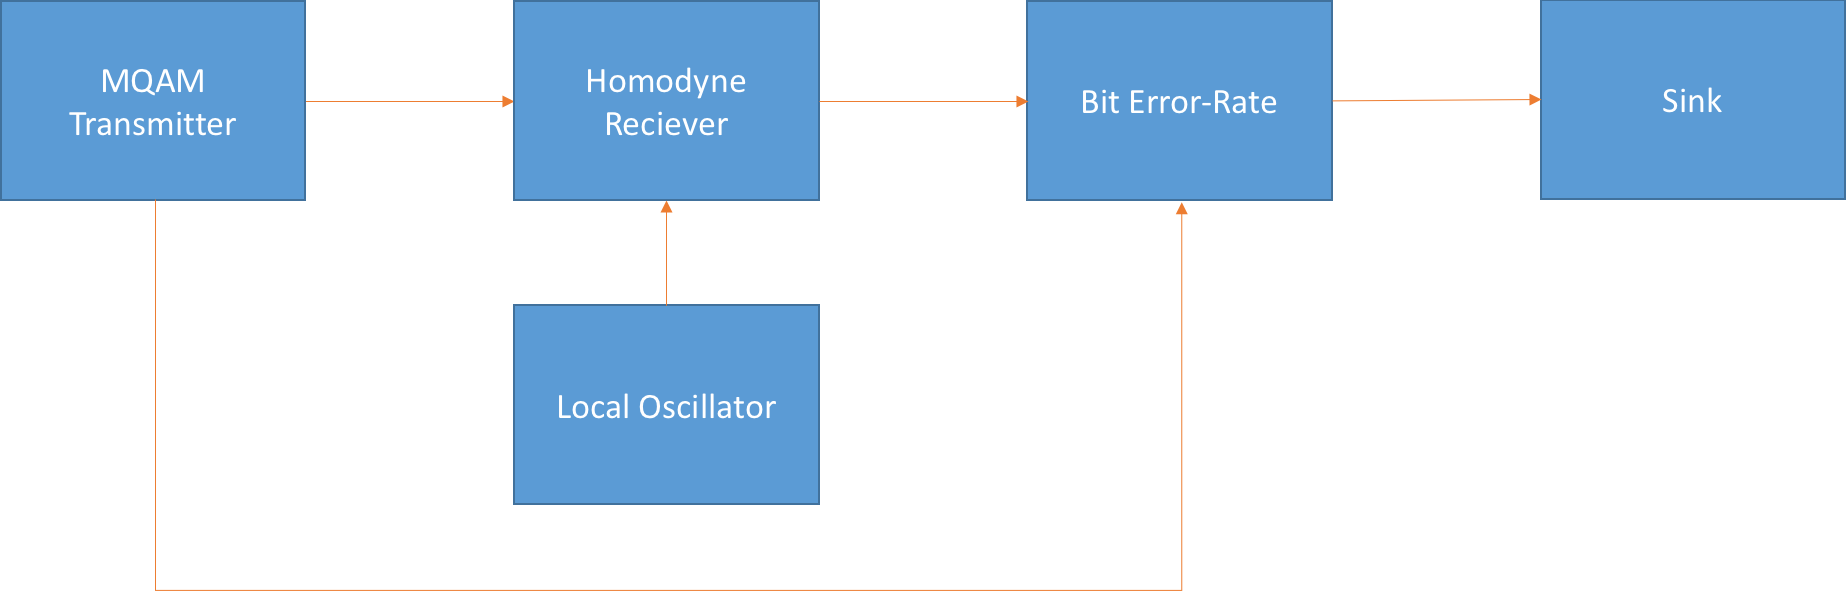
\includegraphics[width=\linewidth]{bpskdiagram.png}
\caption{Overview of the BPSK system being simulated.}
\label{fig:physicalsystem}
\end{figure}

%In the next section we will show that our simulation can currently accomplish all of the proposed objectives.

\section{Simulation Results}

The following results were obtained from the simulation using the following parameters:
\begin{table}[H]
\centering
\begin{tabular}{rl}
NumberOfBits=          & 1000                                                \\
SamplesPerSymbol=      & 16                                                  \\
pLength=               & 5                                                   \\
iqAmplitudesValues=    & \{ \{ 1, 0 \}, \{ -1, 0 \} \}                             \\
outOpticalPower\_dBm=   & -20                                                 \\
LOoutOpticalPower\_dBm= & -10                                                 \\
LocalOscillatorPhase=  & 0                                                   \\
TransferMatrix=        & \{ \{ 1/sqrt(2), 1/sqrt(2), 1/sqrt(2), -1/sqrt(2) \} \} \\
Responsivity=          & 1                                                   \\
Amplification=         & 1e6                                                 \\
NoiseAmplitude=        & 15.397586549153788                                  \\
Delay=                 & 9                                                   \\
\end{tabular}
\end{table}

The system took the binary string presented in Figure~\ref{fig:sentkey} and encoded it into the optical signal in Figure~\ref{fig:sentsig}. Notice the BPSK constelation of the signal, presented in Figure~\ref{fig:constellation}.
\begin{figure}[H]
\centering
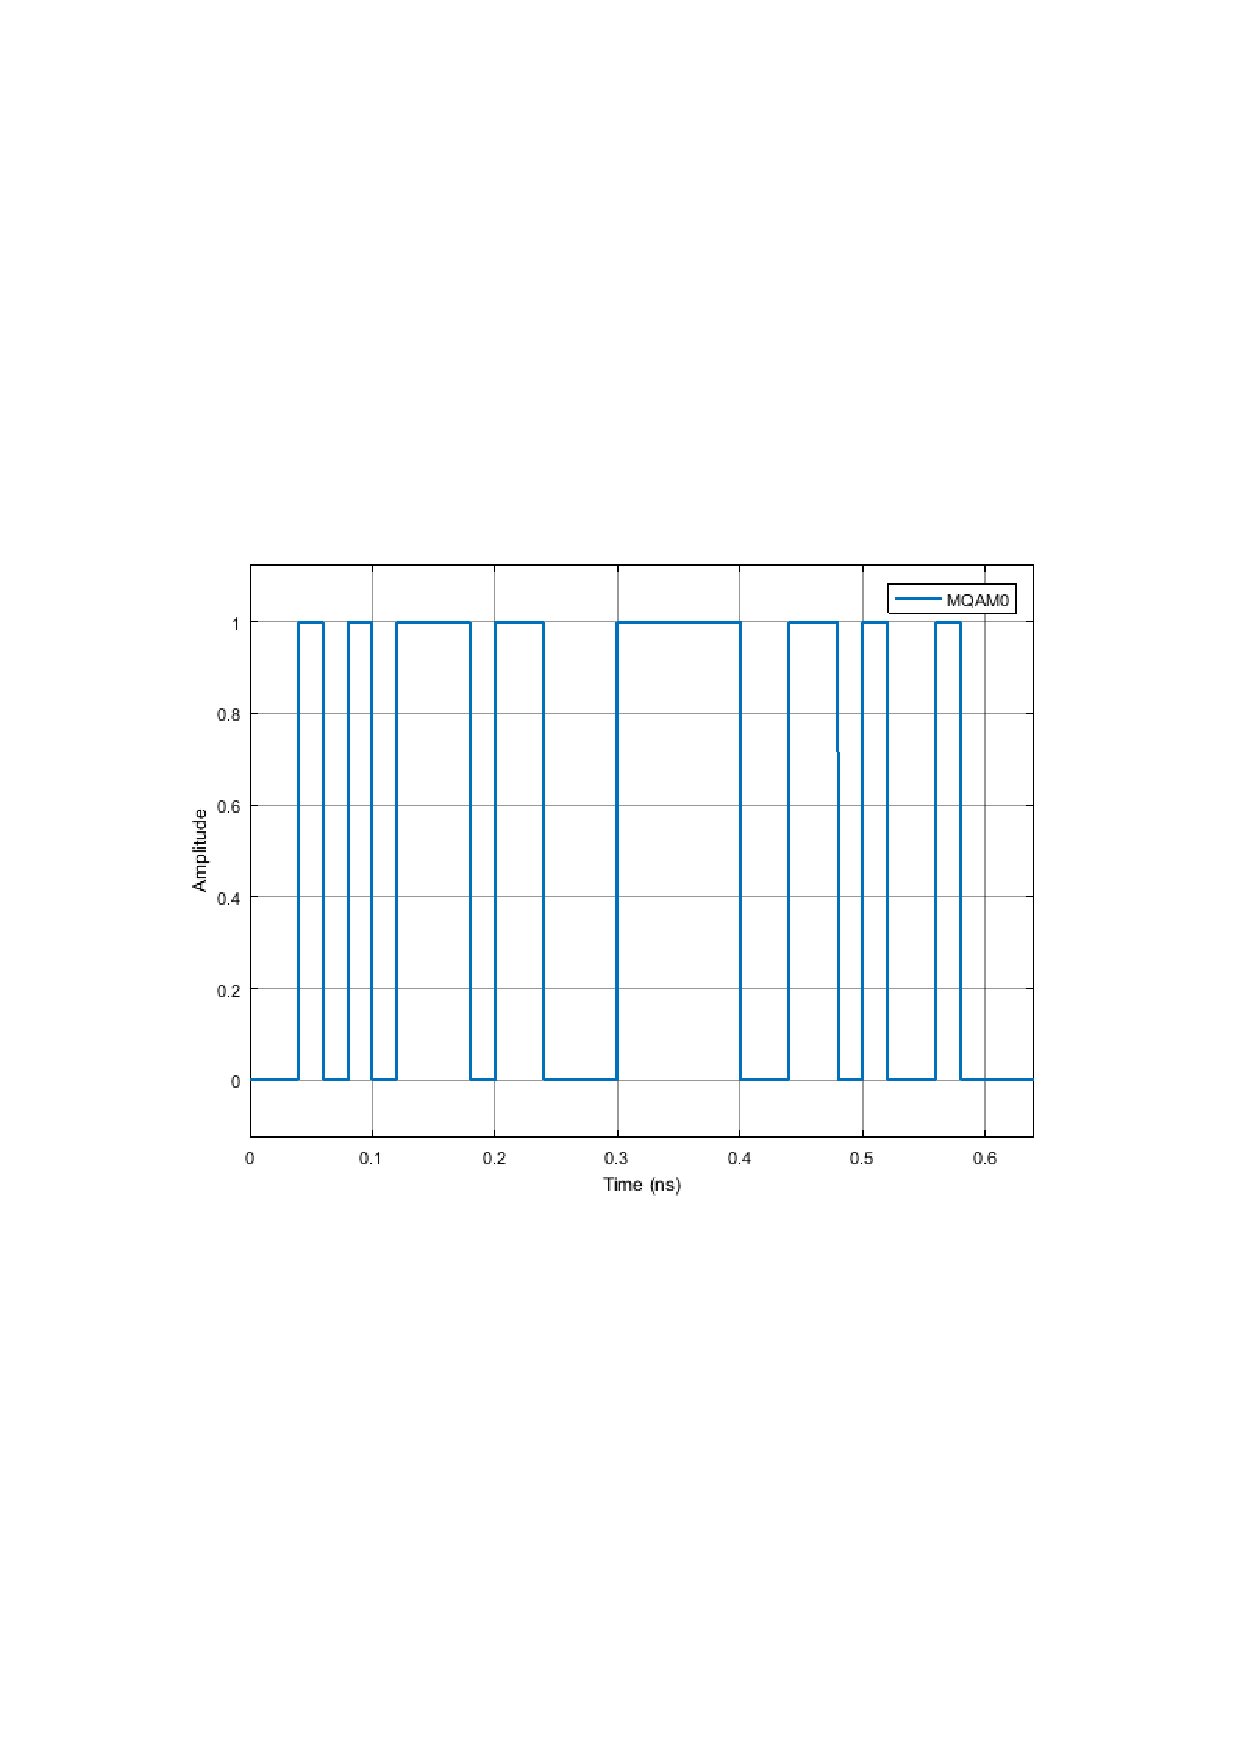
\includegraphics[width=\linewidth, trim= 0mm 95mm 0mm 95mm, clip]{binarystring.pdf}
\caption{Sent binary key.}
\label{fig:sentkey}
\end{figure}

\begin{figure}[H]
\centering
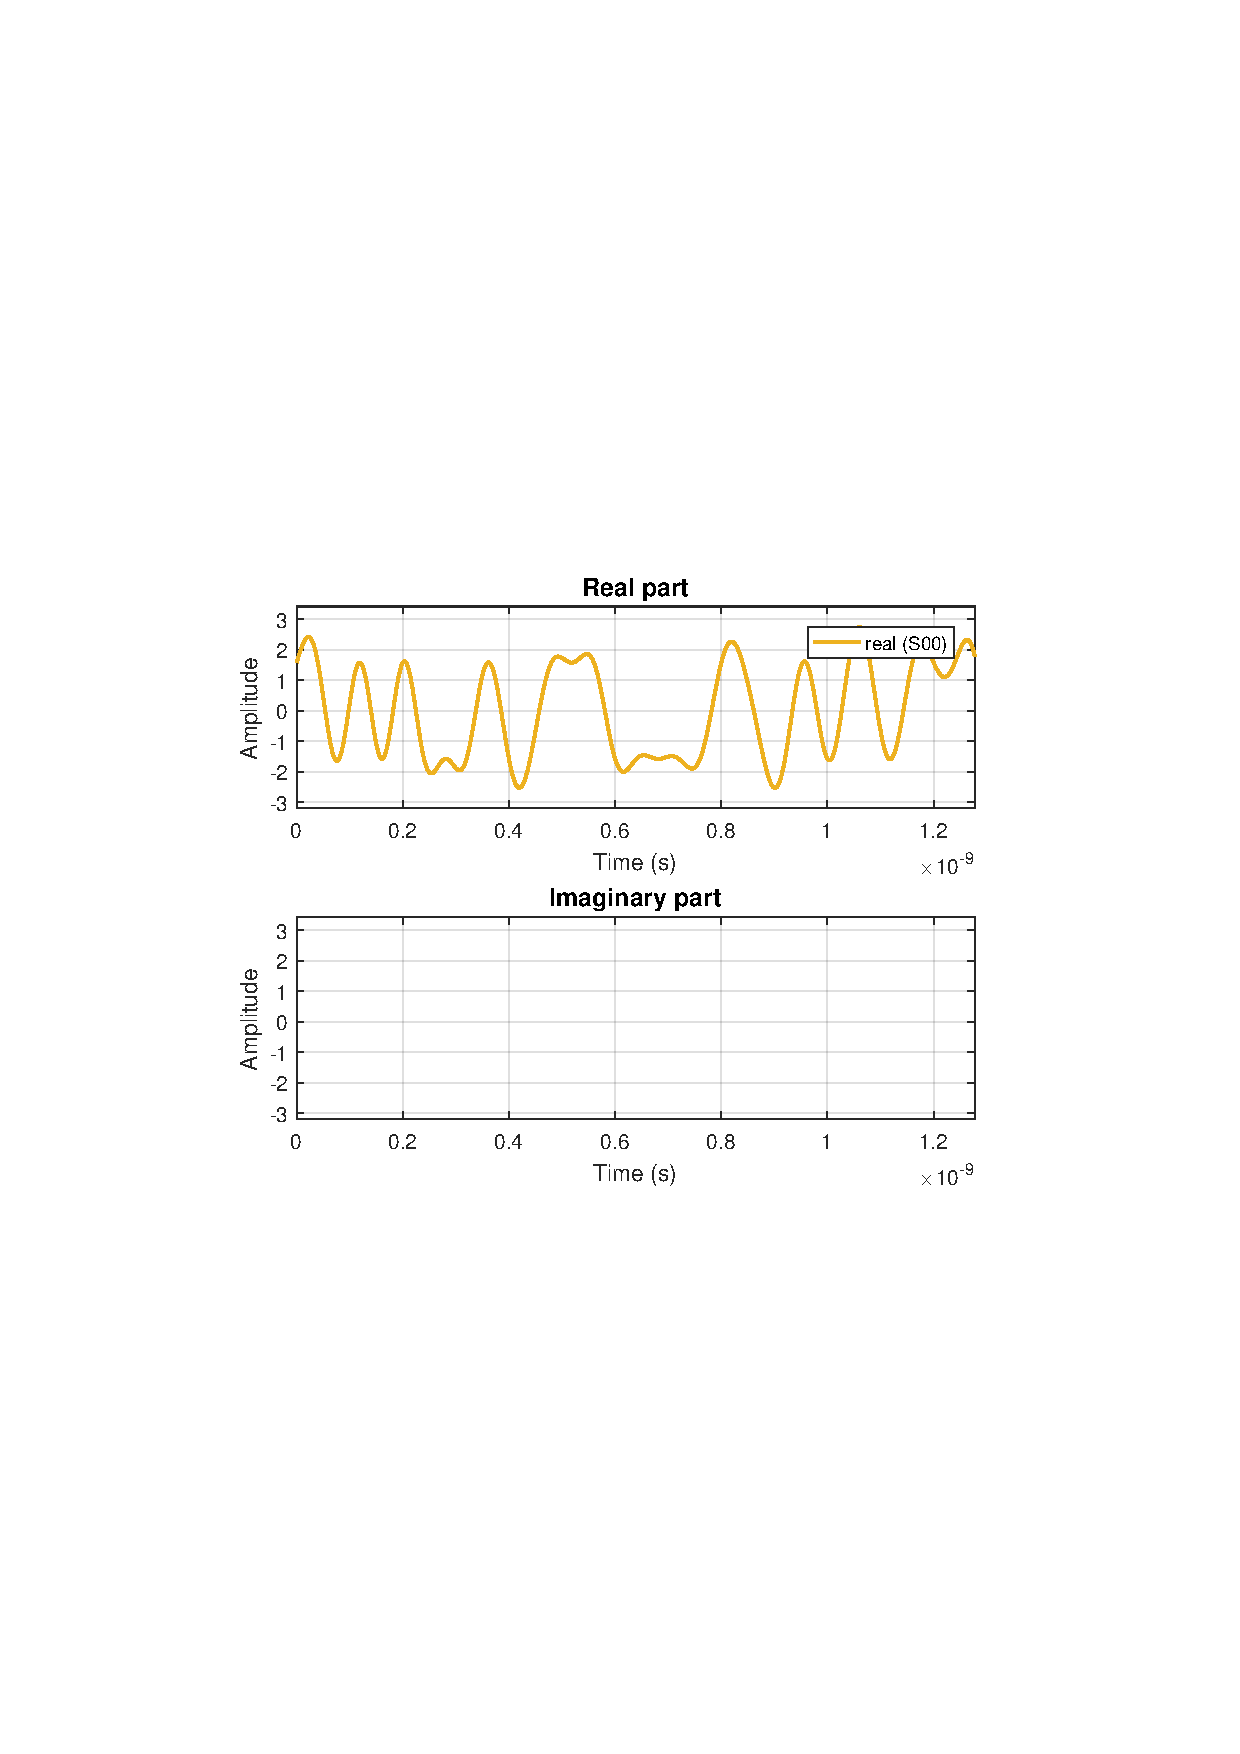
\includegraphics[width=\linewidth, trim= 0mm 95mm 0mm 95mm, clip]{sentsignal.pdf}
\caption{Sent signal.}
\label{fig:sentsig}
\end{figure}

\begin{figure}[H]
\centering
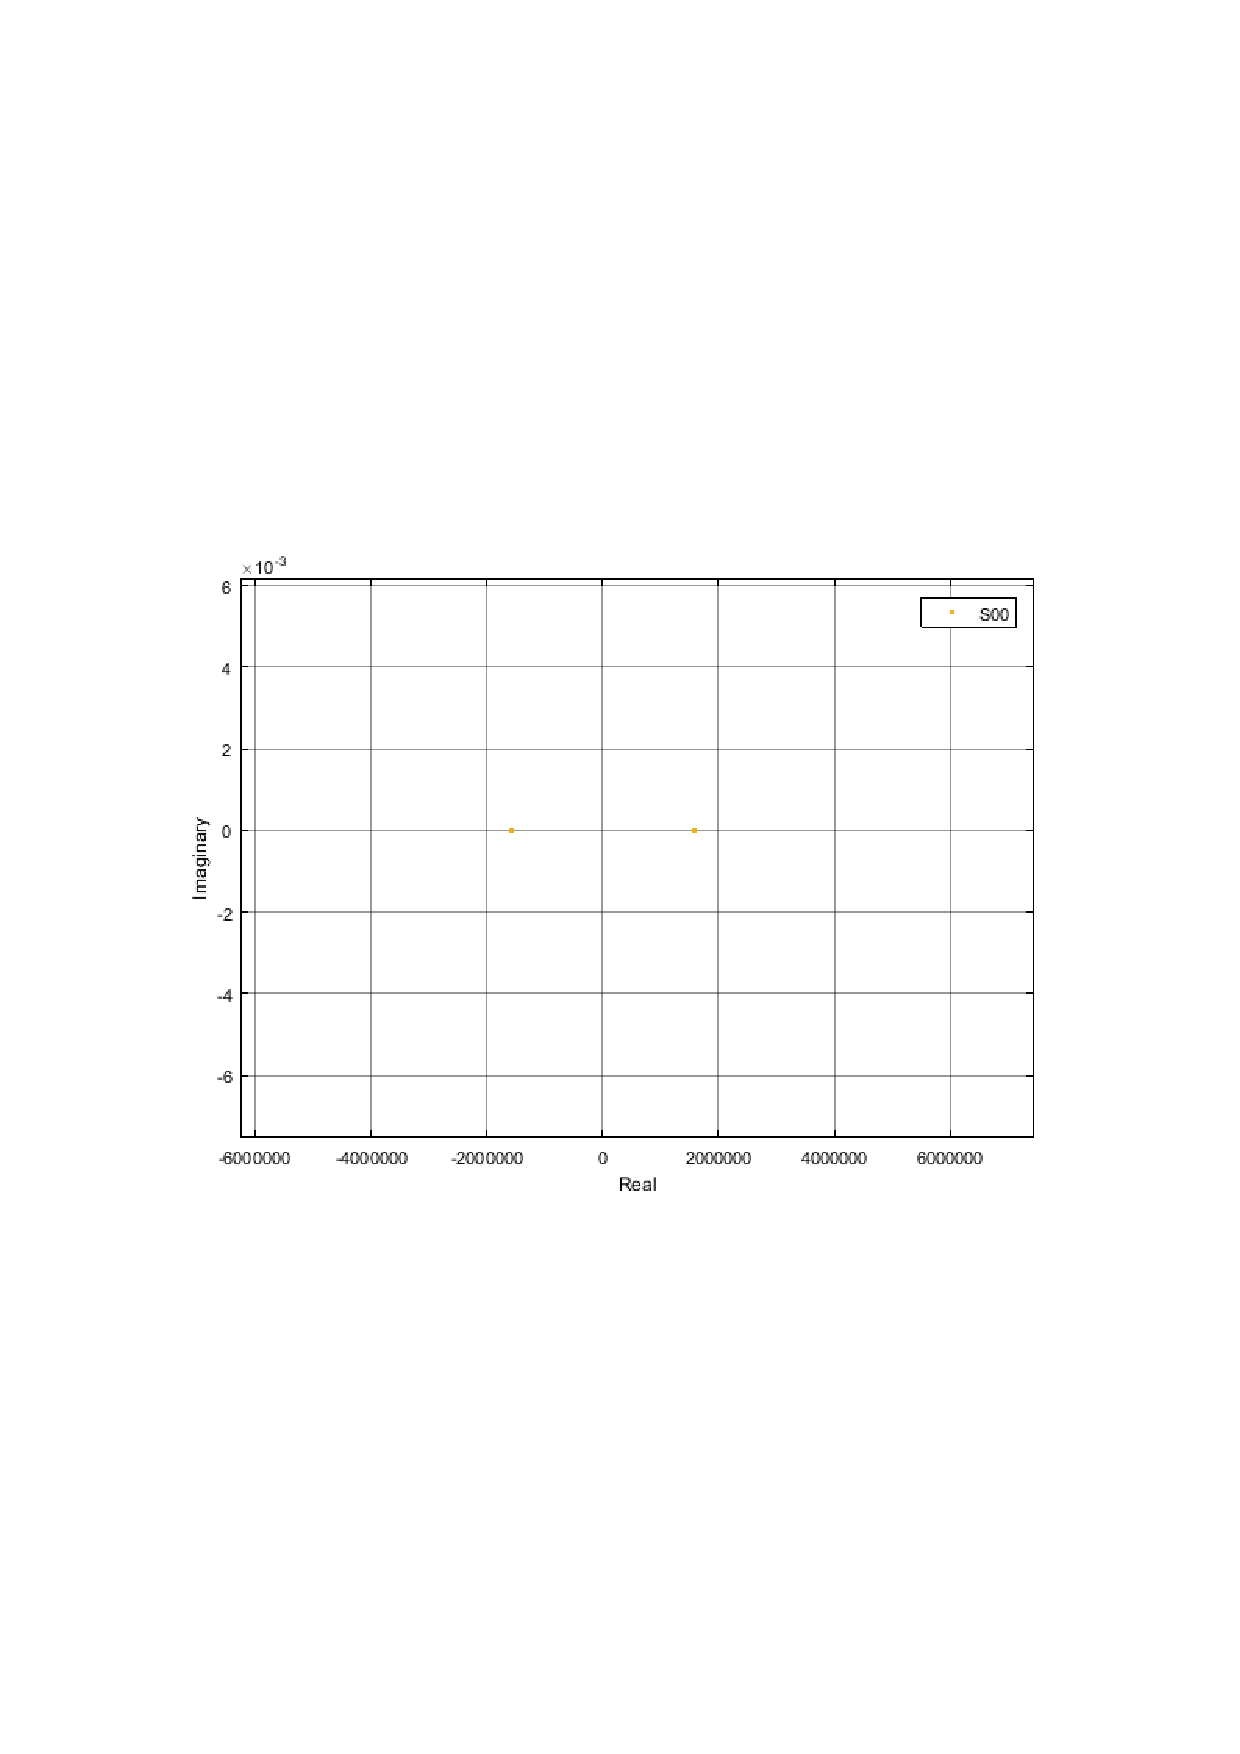
\includegraphics[width=\linewidth, trim= 0mm 95mm 0mm 95mm, clip]{constellation.pdf}
\caption{Constellation of the sent signal.}
\label{fig:constellation}
\end{figure}

Homodyne detection is then performed, using to that effect the local oscillator signal presented in Figure~\ref{fig:local}. Figures~\ref{fig:subtract}~and~\ref{fig:noisy} show the addition of noise to the signal.

\begin{figure}[H]
\centering
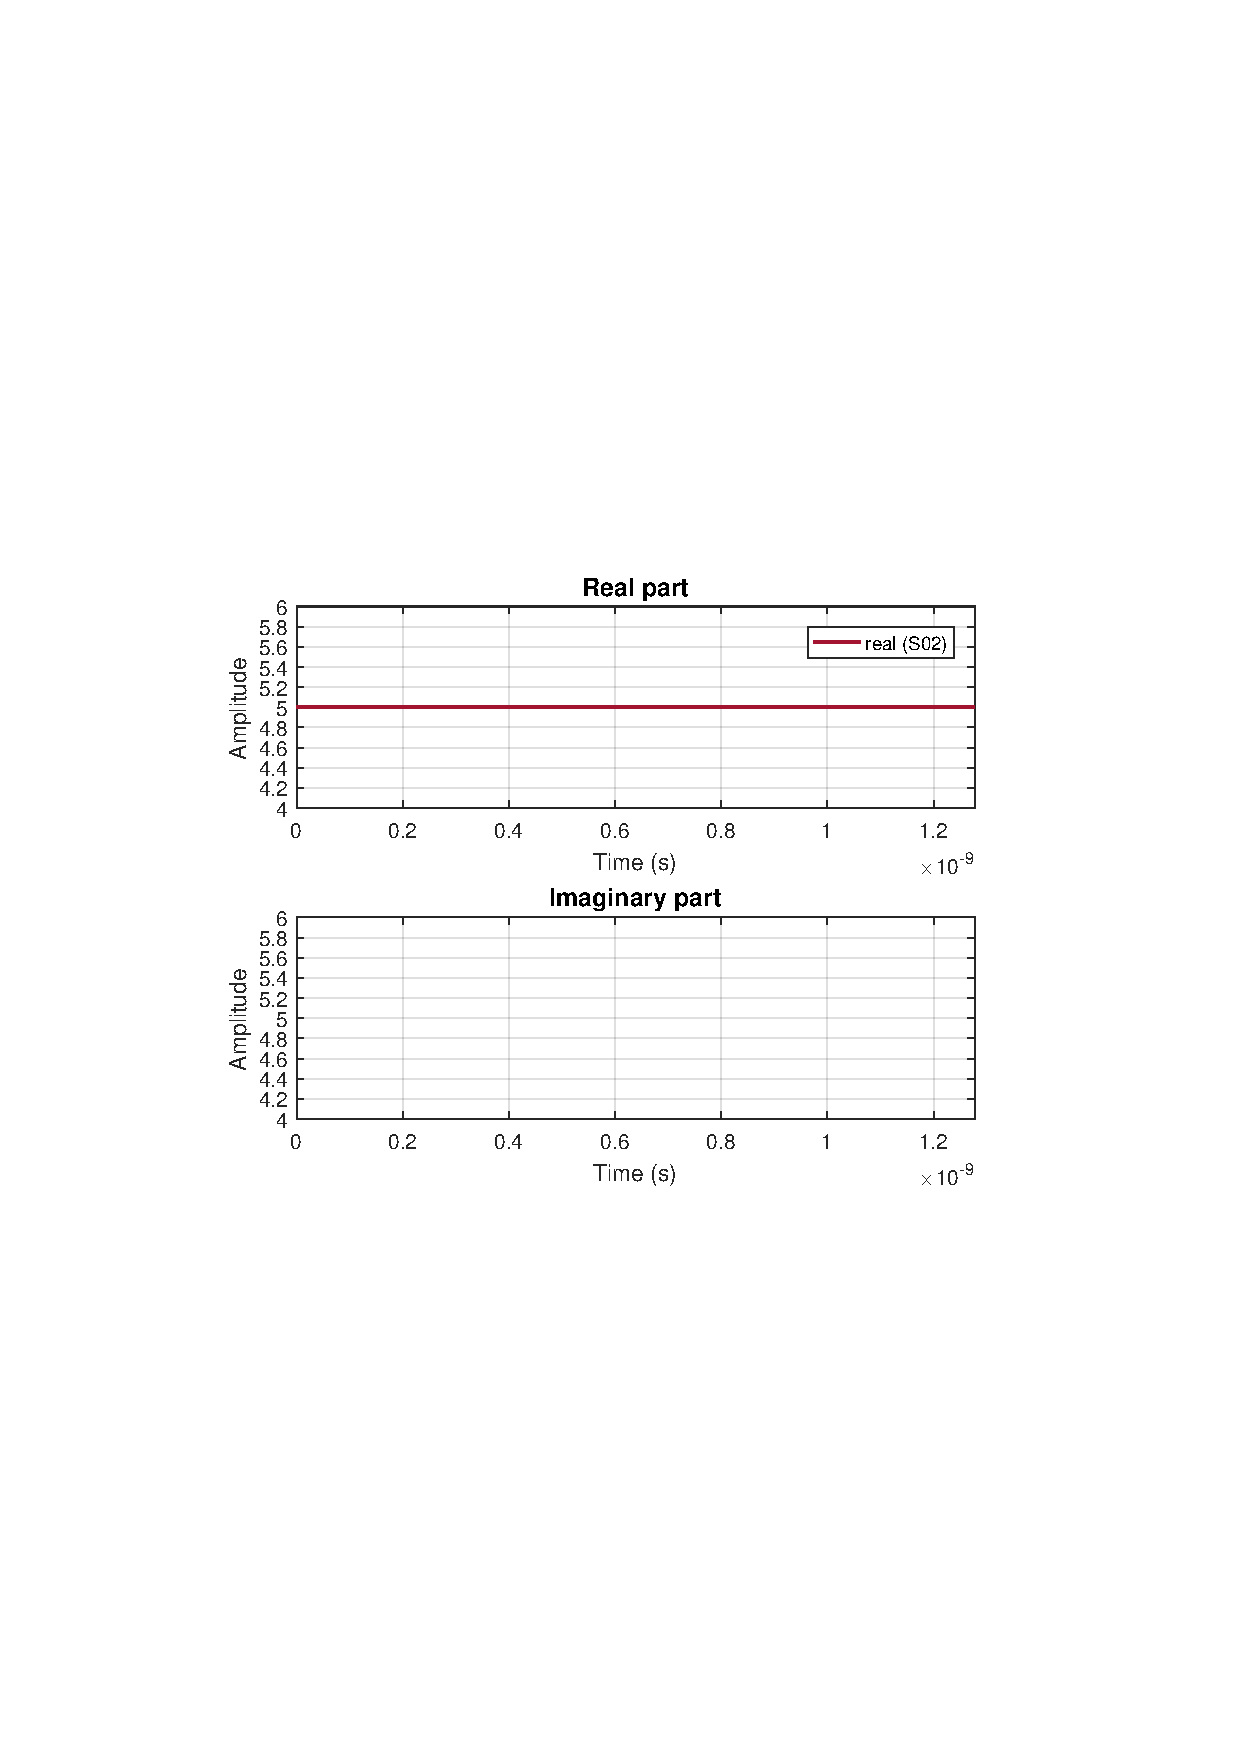
\includegraphics[width=\linewidth, trim= 0mm 95mm 0mm 95mm, clip]{localosc.pdf}
\caption{Homodyne receiver internal signal: local oscillator used for Homodyne detection.}
\label{fig:local}
\end{figure}

\begin{figure}[H]
\centering
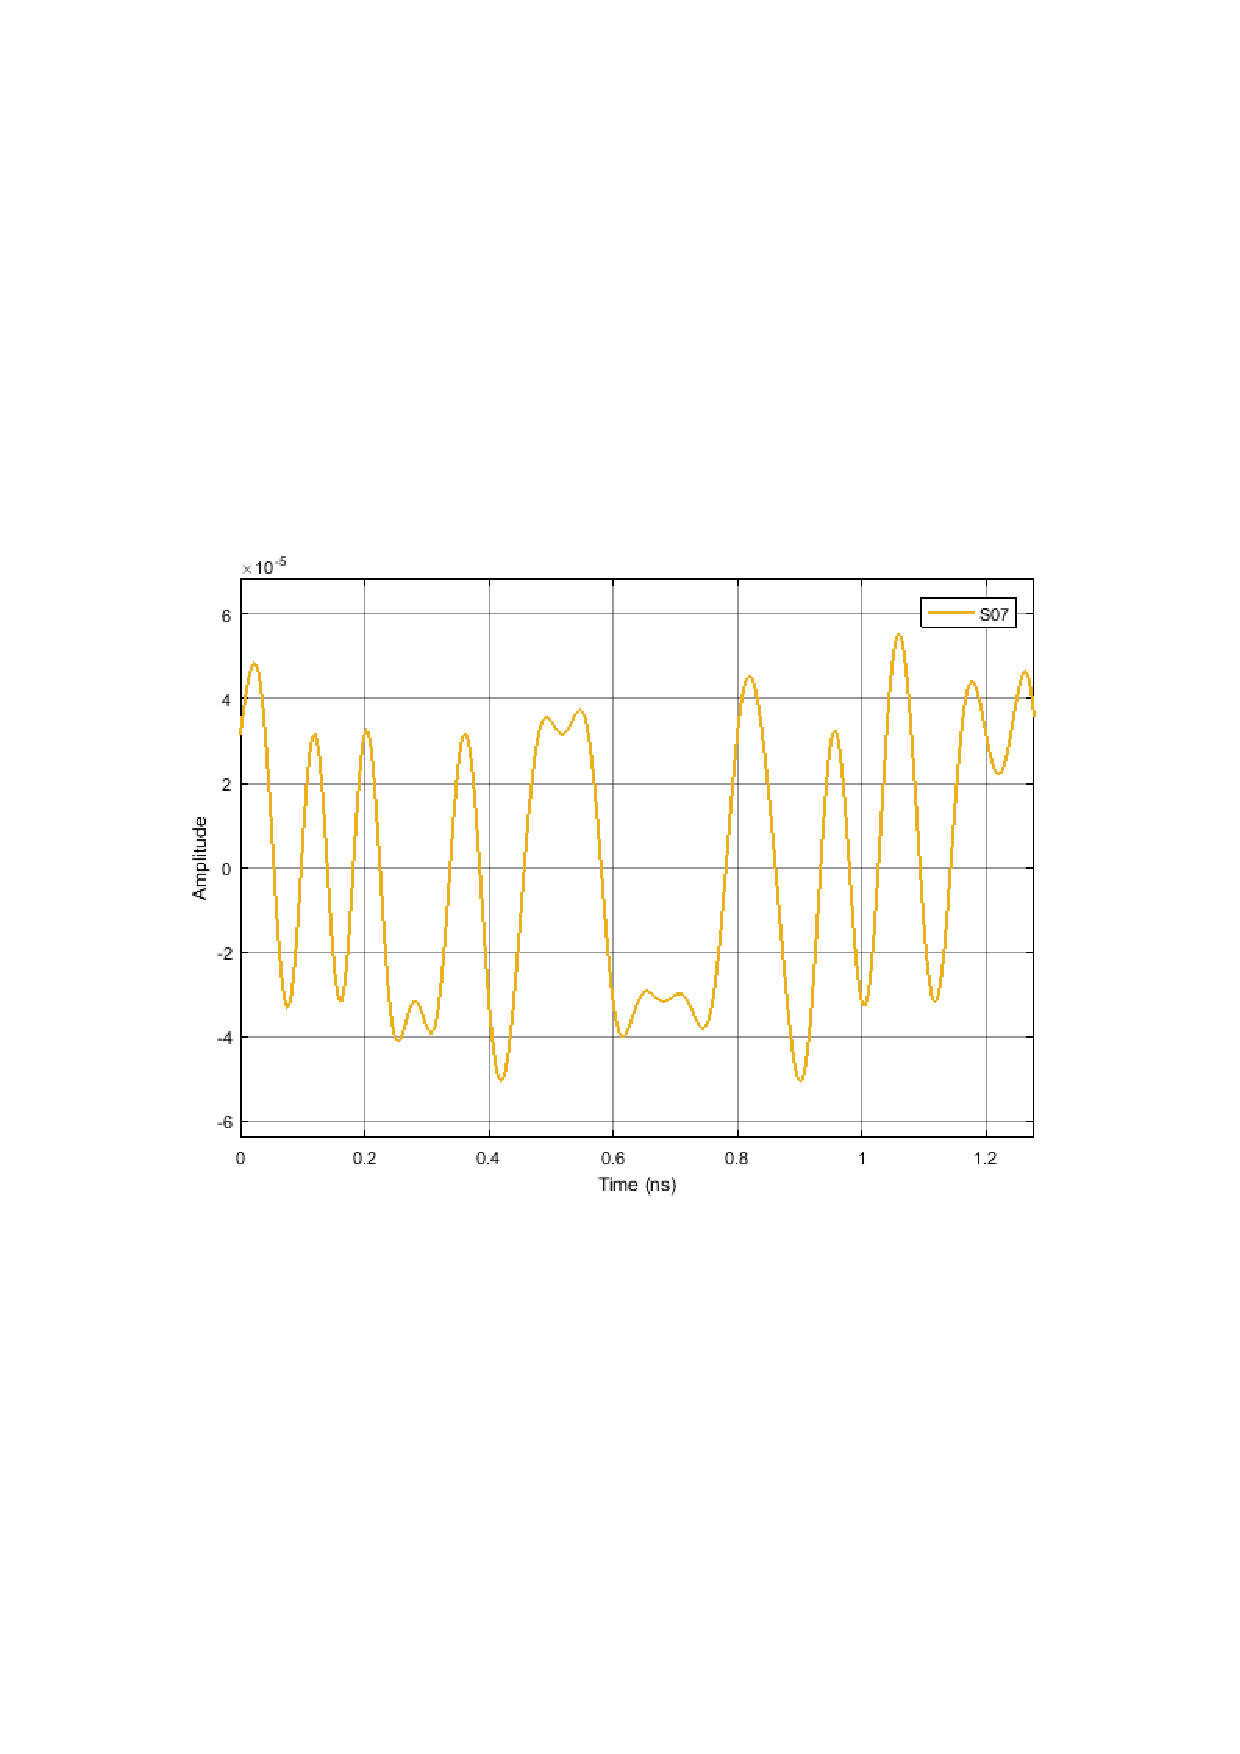
\includegraphics[width=\linewidth, trim= 0mm 95mm 0mm 95mm, clip]{subtract.pdf}
\caption{Homodyne receiver internal signal: subtraction of the signals outputted by the photodiodes.}
\label{fig:subtract}
\end{figure}

\begin{figure}[H]
\centering
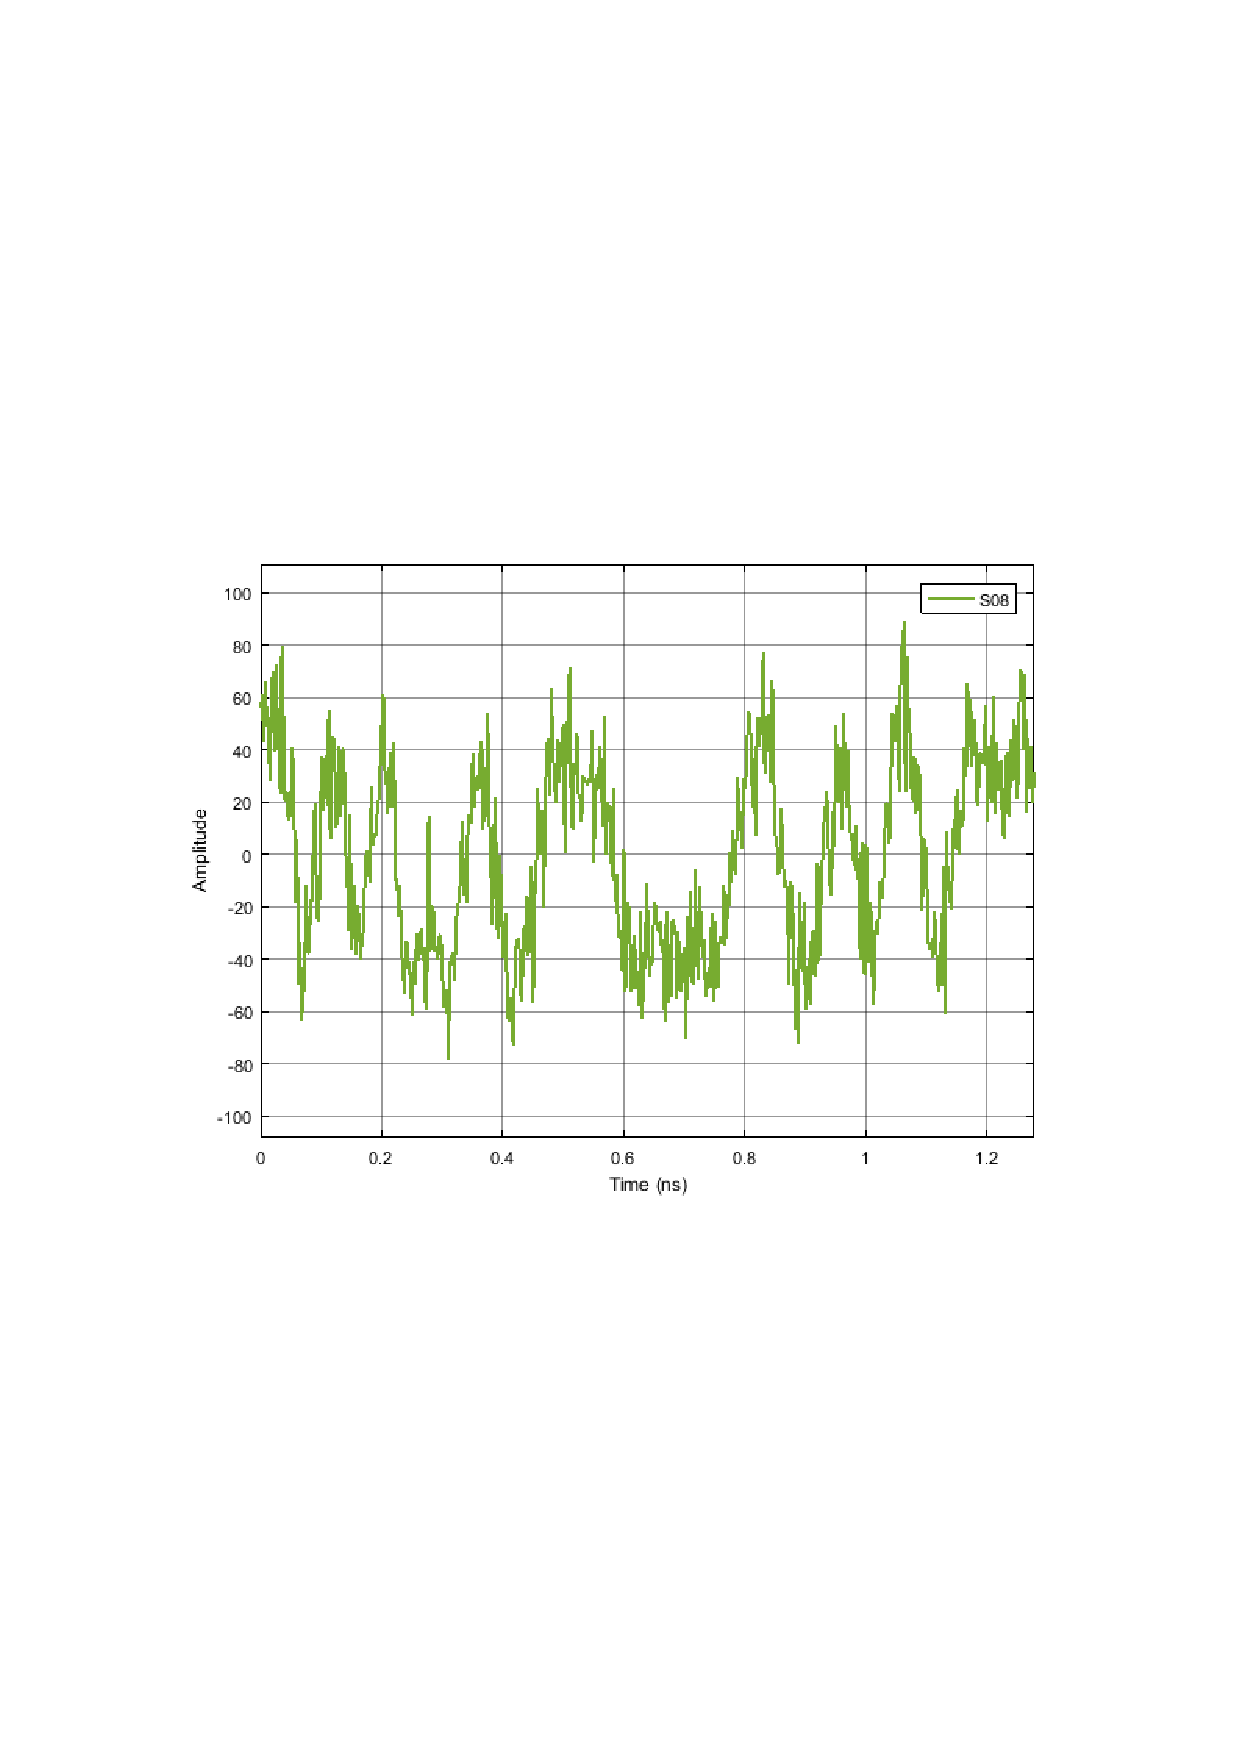
\includegraphics[width=\linewidth, trim= 0mm 95mm 0mm 95mm, clip]{noisy.pdf}
\caption{Homodyne receiver internal signal: amplification of the signal in Figure~\ref{fig:subtract} with added noise.}
\label{fig:noisy}
\end{figure}

The result of the homodyne detection is the binary string presented in~\ref{fig:decoded}, which is then compared to the original binary string by the BER block, which outputs the report presented in Figure~\ref{fig:ber}.

\begin{figure}[H]
\centering
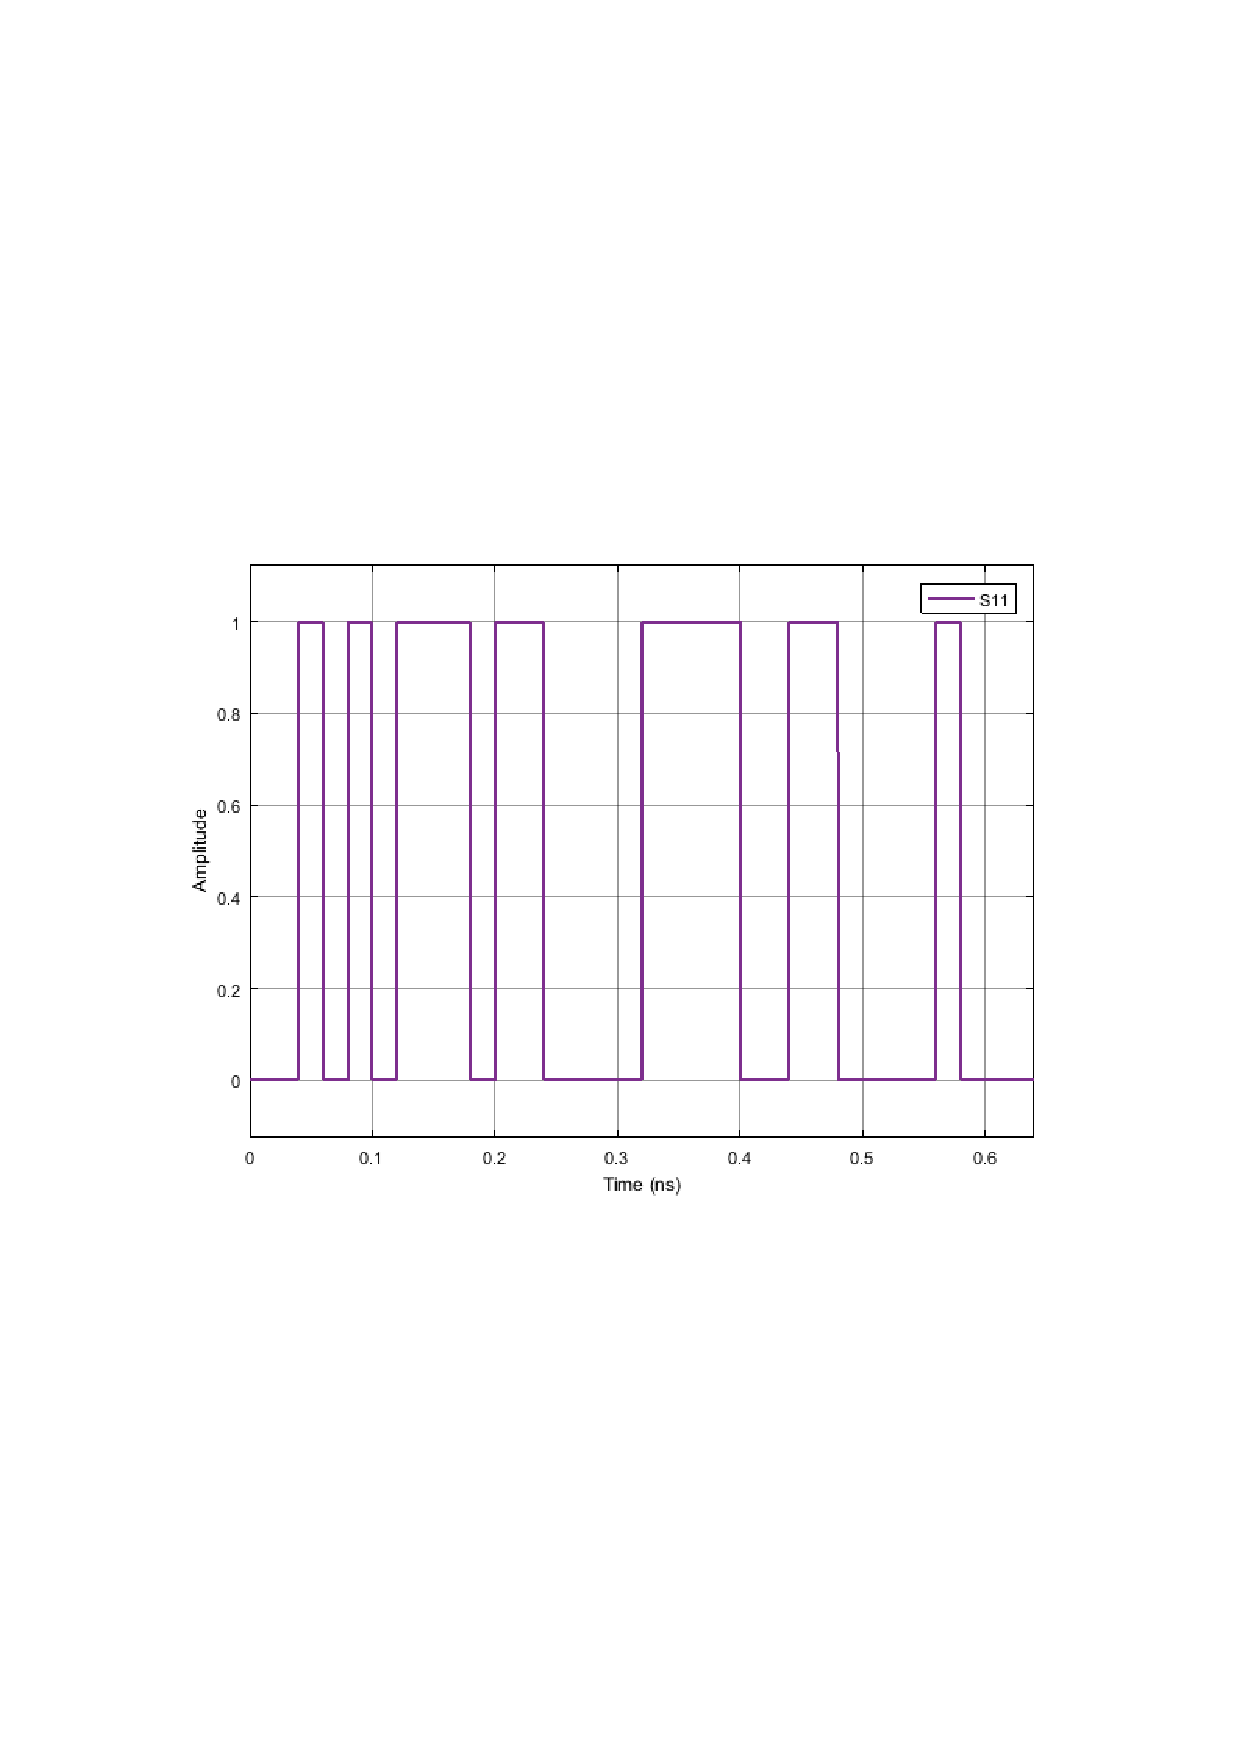
\includegraphics[width=\linewidth, trim= 0mm 95mm 0mm 95mm, clip]{decodedbinarystring.pdf}
\caption{Decoded binary string, output of the Homodyne receiver block.}
\label{fig:decoded}
\end{figure}

\begin{figure}[H]
\centering
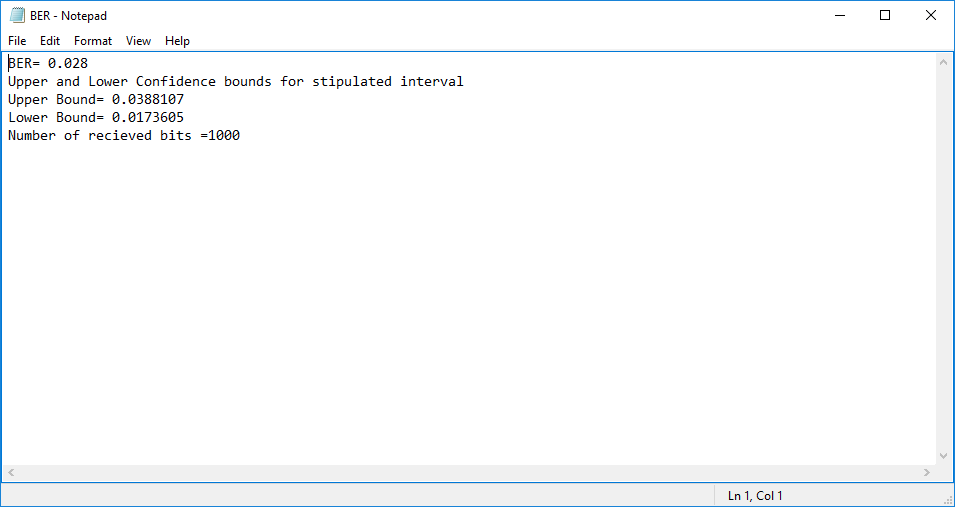
\includegraphics[width=\linewidth]{berreport.png}
\caption{Bit-Error-Rate report.}
\label{fig:ber}
\end{figure}

\pagebreak


\section{Block Description}

\subsection{MQAM Transmitter}
% subfile goes here

\subsection{Homodyne Receiver}
\subfile{../../lib/tex/homodyne_reciever}

\subsection{Bit Error-Rate}
\subfile{../../lib/tex/ber}

\end{document}